\chapter{Методы исследования аттракторов внутренних волн}

Качественно, аттракторы внутренних волн, возникающие после многократной фокусировки в акватории, выражаются в повышенной интенсивности движения стратифицированной жидкости около геометрического контура фокусировки. Первичный способ изучить форму аттрактора -- это метод трассировки лучей \cite{Maas1997}. Этот метод помогает при в поиске аттракторов в акваториях с различными геометрическими характеристиками \cite{Guo2015}. Метод трассировки лучей дает ответ на вопрос о принципиальном существовании аттрактора в конкретной геометрии. Однако, Этот метод не дает данных о поле скорости вблизи аттрактора и не учитывает вязкость жидкости, в которой это явление может возникать.

Получение количественных характеристик аттрактора внутренних волн невозможно без использования экспериментальных установок или численного моделирования \cite{Brouzet2016}. Экспериментальными исследованиями аттракторов внутренних волн впервые начал заниматься Лео Маас с 1997 года \cite{Maas1997}. В 2011 году была построена установка в Массачусетском технологическом университете и проведены серии экспериментов \cite{Hazewinkel2011} после сотрудничества с Лео Маасом \cite{Hazewinkel2010}. Сейчас экспериментальным исследованием аттракторов занимаются Терри Доксуа \cite{Dauxoisetal2018} во Франции, а в России -- Евгений Ерманюк \cite{brouzet1997laboratory}.

Наиболее точным методом численного моделирования аттракторов внутренних волн является метод спектральных элементов \cite{NEK5000}. Разница с экспериментом составила всего 10\% \cite{Brouzet2014}. Однако, у него имеются свои недостатки о которых упоминается в этой главе. Альтернативой методу спектральных элементов служит метод конечных элементов \cite{ferziger2002computational} и широко используемые в рамках этого метода алгоритм PISO \cite{Issa1986-PISO}. Алгоритм PISO также не лишен недостатков о которых будет сказано позднее. Еще одной альтернативой является квазигидродинамический подход и регуляризированные уравнения \cite{ElizarBook}. Предполагается, что такой подход при сохранении удобства использования и модификации методов будет обладать повышенной точностью. 

\section{Исследование свойств волновых течений с помощью трассировки лучей}

В предыдущей главе уже была затронута тема трассировки лучей. Это геометрическое представление пучков внутренних волн в виде лучей \cite{Maas1995}, которые отражаются от поверхностей согласно дисперсионному соотношению (\ref{eq:dispersion}).

Прослеживая траекторию лучей в замкнутом трапециевидном резервуаре можно определить будет ли при данных геометрических параметрах и частоте волнопродуктора образовываться аттрактор внутренних волн. Каждое отражение от наклонной стенки увеличивает амплитуду фазовой скорости внутренней волны, но уменьшает ее длину. На существование и форму аттрактора влияют несколько факторов:

\begin{itemize}
    \item Угол наклона фокусирующей поверхности ($\alpha$)
    \item Частота плавучести $N$
    \item Частота колебаний волнопродуктора $\omega$
    \item Длинна резервуара $L_1$
    \item Высота резервуара $H$
\end{itemize}

Для простоты рассмотрим трапециевидный резервуар 

\begin{figure}[!ht]
    \centering
    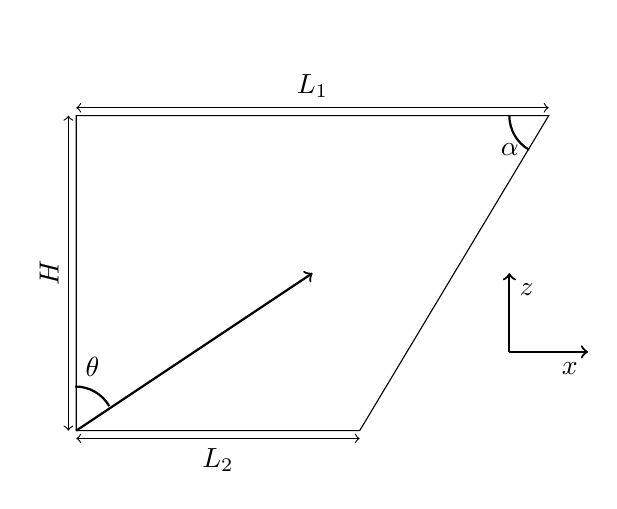
\begin{tikzpicture}[scale=1, z={(-.707,-.5)}]
    \draw (3.6,0,0) -- (0,0,0) -- (0,4,0)--(6,4,0)--(3.6,0,0);
    %\draw (3.6,0,0) -- (3.6,0,-1) -- (6,4,-1) -- (6,4,0) -- cycle;
    %\draw (6,4,0) -- (0,4,0) -- (0,4,-1) -- (6,4,-1);
    \draw (-0.5,2,0) node{};
    \draw (4.1,-.2,-1.5) node{};
    \draw (3.5,5,0) node{};
    \draw[<->] (-0.1,0) --node[above,rotate=90] {$H$} (-0.1,4);
    \draw[<->] (0,4.1,0) --node[above,] {$L_1$} (6,4.1,0);
    \draw[<->] (0,-0.1,0) --node[below,] {$L_2$} (3.6,-0.1,0);
    \draw [black, thick] (5.5,4) arc [start angle=180, end angle=240, radius=0.5cm]
        node [left] {$\alpha$};
    \draw[thick,->] (5.5,1,0) -- (6.5,1,0) node[anchor=north east]{$x$};
    \draw[thick,->] (5.5,1,0) -- (5.5,2,0) node[anchor=north west]{$z$};
    \draw[thick,->] (0,0,0) -- (3,2,0) ;

    \draw [black, thick] (0.42,0.31) arc [start angle=30, end angle=90, radius=0.5cm] node [above right] {$\theta$};
    
    \end{tikzpicture}
    \caption{Область фокусировки лучей внутренних волн, где $\theta = sin \frac{\omega}{N}$}
    \label{fig:domainup}
\end{figure}

Задачу трассировки лучей можно упростить, введя параметры. В своей работе он предлагает параметризовать резервуар фокусировки внутренних волн следующим образом(Рис. \ref{fig:domainTran}):

Применяется преобразование горизонтальной координаты, которое перемещает систему координат таким образом чтобы левый конец резервуара соответствовал координате $-1$ а правый $1$. Вводится параметр $d$ который обозначает расстояние от нуля новой горизонтальной оси до точки соприкосновения наклонной стенки с горизонтальной осью.
\begin{equation}
    x'=\frac{x\cdot 2}{L_1}-1
    \label{eq:transformX}
\end{equation}

Затем преобразование вертикальной координаты, которое сжимает или растягивает высоту резервуара так, чтобы угол отражения и распространения внутренних волн стал $45^\circ$. При этом вводится параметр $\tau$, который обозначает новую высоту резервуара. 
\begin{equation}
    z'=\frac{z\cdot 2}{L_1}\sqrt{\frac{N^2}{\omega^2}-1}
    \label{eq:transformZ}
\end{equation}

Таким образом вместо пяти определяющих параметров для геометрической задачи, остаются всего два, $d$ и $\tau$.

Благодаря методу трассировки лучей можно геометрически предсказать форму аттрактора внутренних волн. 

\begin{figure}
    \begin{subfigure}{\textwidth}
    \centering
    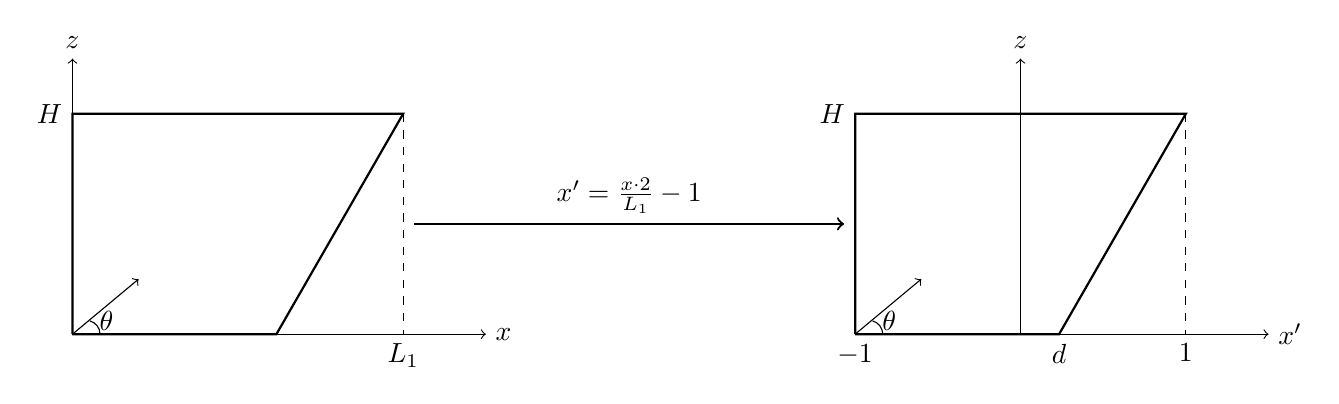
\begin{tikzpicture}[scale=0.7]
        \draw[thick] (0,0)--(0,4)node[left]{$H$}--(6,4)--(3.7,0)--(0,0);
        \draw[dashed] (6,4) -- (6,0)node[below]{$L_1$};
        \draw[thick,->] (6.2,2)->node[above]{$x'=\frac{x\cdot 2}{L_1}-1$}(14,2);
        \draw[->] (0,0)->(0,5)node[above]{$z$};
        \draw[->] (0,0)->(7.5,0)node[right]{$x$};
        \draw[->] (0,0)->(1.2,1);
        \draw[black] (0.5,0) arc [start angle=0, end angle=75, radius=0.25cm] node [right] {$\theta$};
        \draw[thick] (14.2,0)node[below]{$-1$}--(14.2,4)node[left]{$H$}--(20.2,4)--(17.9,0)node[below]{$d$}--(14.2,0);
        \draw[dashed] (20.2,4) -- (20.2,0)node[below]{$1$};
        \draw[->] (17.2,0)->(21.7,0)node[right]{$x'$};
        \draw[->] (17.2,0)->(17.2,5)node[above]{$z$};
        \draw[->] (14.2,0)->(15.4,1);
        \draw [black] (14.7,0) arc [start angle=0, end angle=75, radius=0.25cm] node [right] {$\theta$};
    \end{tikzpicture}
    \caption{Горизонтальное преобразование расчетной области}
    \end{subfigure}
    
    \begin{subfigure}{\textwidth}
    \centering
    \begin{tikzpicture}[scale=0.7]
        \draw[thick] (0,0)--(0,4)node[left]{$H$}--(6,4)--(3.7,0)--(0,0);
        \draw[dashed] (6,4) -- (6,0)node[below]{$L_1$};
        \draw[thick,->] (6.2,2)->node[above]{$z'=\frac{z\cdot 2}{L_1}\sqrt{\frac{N^2}{\omega^2}-1}$}(14,2);
        \draw[->] (0,0)->(0,5)node[above]{$z$};
        \draw[->] (0,0)->(7.5,0)node[right]{$x$};
        \draw[thick] (14.2,0)--(14.2,4.8)node[left]{$\tau$}--(20.2,4.8)--(17.9,0)--(14.2,0);
        \draw[black] (0.5,0) arc [start angle=0, end angle=75, radius=0.25cm] node [right] {$\theta$};
        \draw [black] (14.7,0) arc [start angle=0, end angle=80, radius=0.25cm] node [right] {$45^\circ$};
        \draw[->] (0,0)->(1.2,1);
        \draw[->] (14.2,0)->(15.4,1.2);
        \draw[dashed] (20.2,4.8) -- (20.2,0)node[below]{$L_1$};
        \draw[->] (17.2,0)->(21.7,0)node[right]{$x$};
        \draw[->] (14.2,0)->(14.2,6)node[above]{$z'$};
    \end{tikzpicture}
    \caption{Вертикальное преобразование расчетной области}
    \end{subfigure}
    \caption{Преобразования расчетной области для процедуры получения диаграммы Мааса}
    \label{fig:domainTran}
\end{figure}

На рисунке \ref{fig:RayTr923x1455} изображен резервуар до перехода и после перехода к параметрам $(d,\tau)$.

\begin{figure}
    \begin{subfigure}[с]{0.45\textwidth}
        \centering
        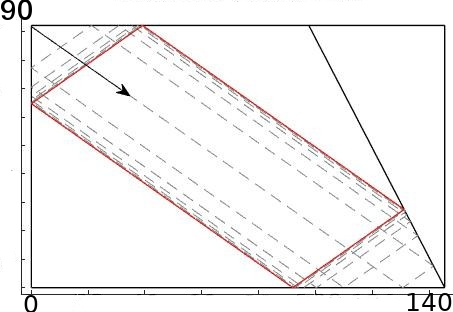
\includegraphics[scale=0.45]{Figs/RayTr923x1455.jpeg}
        \caption{Трассировка лучей,\\ $H=92.3$, $L=145.5$, $\theta = 35.13^{\circ}$,\\ $\alpha = 27.4^{\circ}$}
    \end{subfigure}
    \begin{subfigure}[r]{0.45\textwidth}
        \centering
        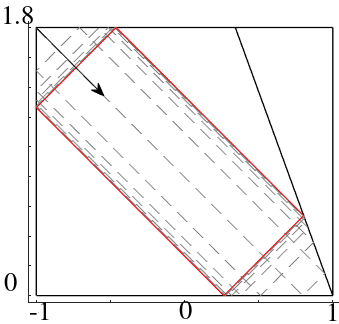
\includegraphics[scale=0.45]{Figs/RTdtau.png}
        \caption{Трассировка лучей в преобразованной геометрии, \\ $\tau = 1.8$, $d = 0.34$}
    \end{subfigure}
    
    \caption{Результат работы процедуры трассировки лучей и результат перехода к параметрам $(d,\tau)$}

    \label{fig:RayTr923x1455}
\end{figure}

После преобразования можно перейти в плоскость параметров и отобразить цветом среднюю кинетическую энергию в резервуаре \cite{Maas1997} и области формирования аттрактора внутренних волн. Средняя кинетическая энергия в резервуаре получена прямым численным моделированием (Рис. \ref{fig:diagramm}). 

\begin{figure}
    \centering
    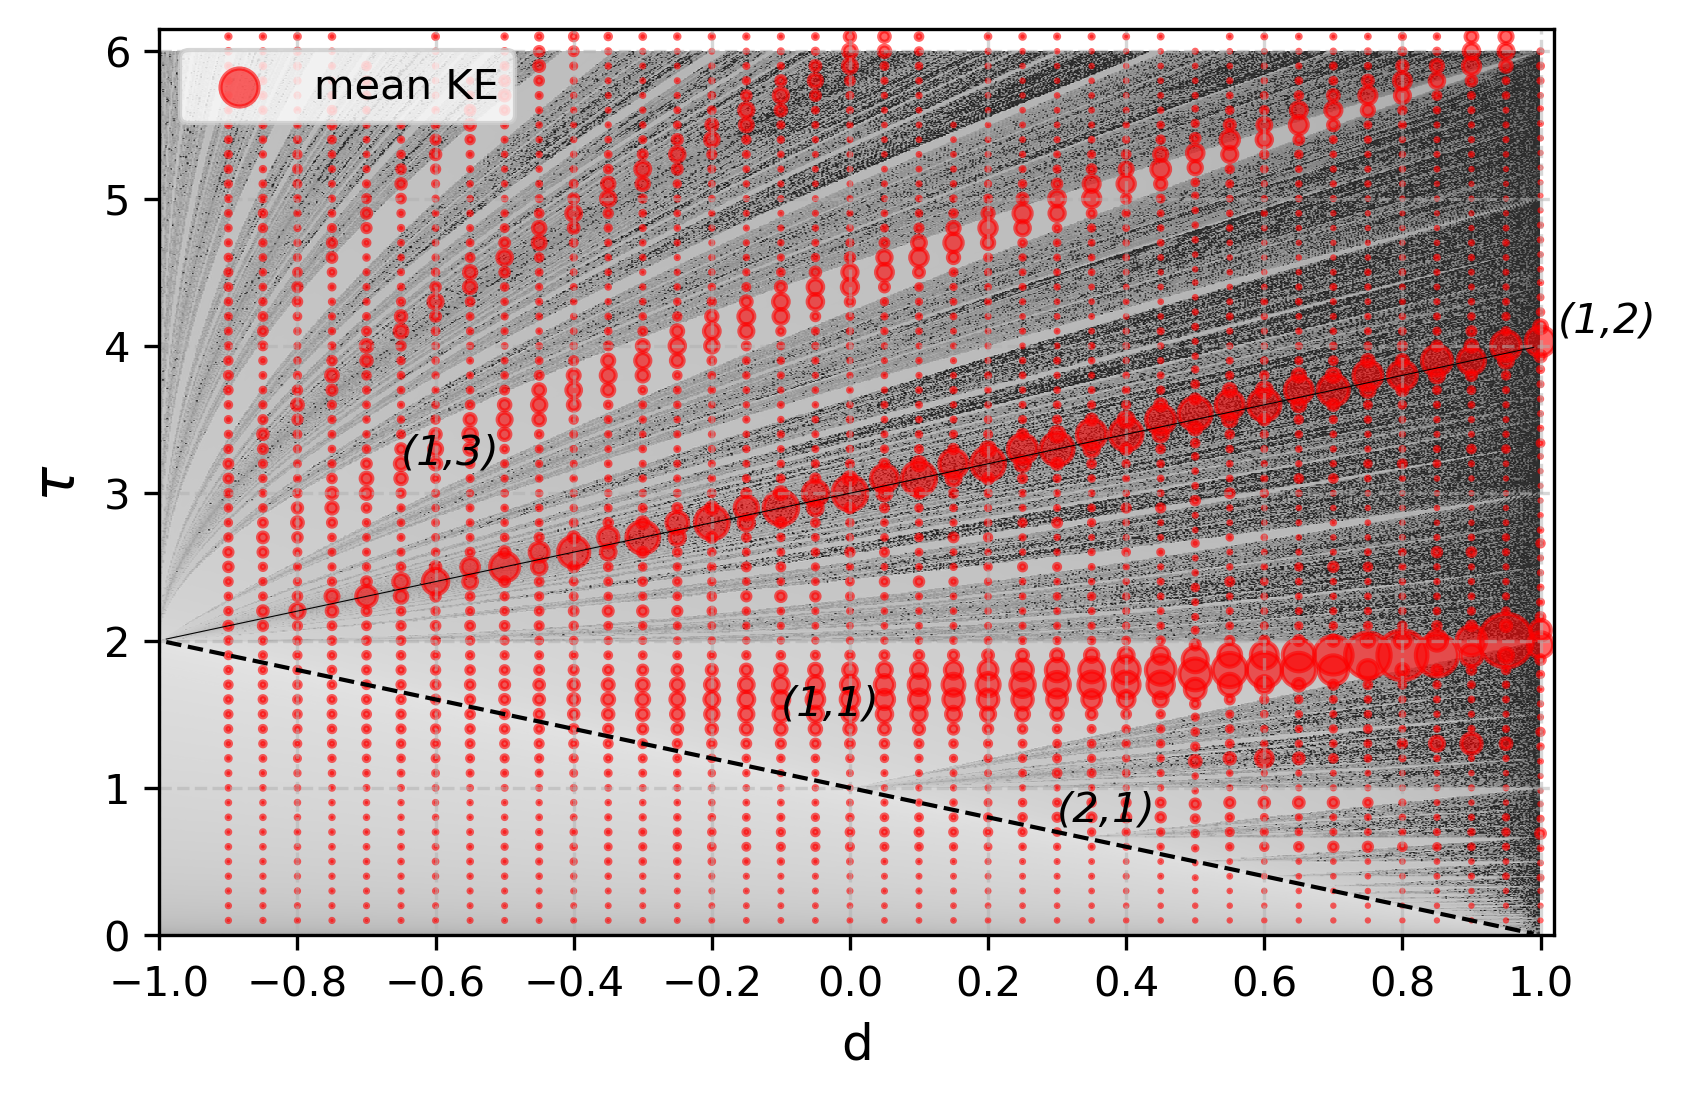
\includegraphics{pics/KEandLyap.png}
    \caption{Средняя кинетическая энергия во множестве резервуаров, в координатах ($\tau$,$d$). Величина точки показывает относительное количество кинетической энергии в резервуаре. Светлые области -- области существования аттрактора. }
    \label{fig:diagramm}
\end{figure}

\subsection{Критические частоты и диапазон существования аттракторов внутренних волн}

В этой работе рассматривается зона существования аттракторов помеченная на рисунке \ref{fig:diagramm} маркером $(1,1)$. Влиять на параметр $d$ можно изменяя геометрические характеристики резервуара. А параметр $\tau$ регулируется изменением частоты колебаний волнопродуктора. Если изменяется параметр $\tau$, или просто $\omega$, то изменяется и форма аттрактора внутренних волн. Аналитически можно получить диапазон частот в зависимости от геометрических параметров резервуара, который определит существование аттрактора или его отсутствие при данных параметрах.

Найдем такие параметры системы, чтобы аттрактор вырождался в отрезки для этого положим $\tau=2$. Выбор такого значения обусловлен углом распространения внутренних волн $\theta = 45^{\circ}$. Это значит, что волна пущенная из левого верхнего угла упрется в правый нижний угол так как длинна резервуара $=2$ от $-1$ до $1$(см рис. \ref{fig:trivAttr}). Если в уравнение (\ref{eq:transformZ}) подставить вместо $z$ высоту резервуара $H$ то получим:

\begin{equation}
    \tau=\frac{2H}{L} \sqrt{\frac{N^2}{\omega^2}-1}.
\end{equation}

Теперь подставим $\tau=2$:

\begin{equation}
    1=\frac{H}{L} \sqrt{\frac{N^2}{\omega^2}-1}.
\end{equation}

Выразим отсюда $\omega$:

\begin{equation}
    \omega=\frac{NH}{\sqrt{L^2+H^2}}.
\end{equation}

\begin{figure}
    \centering
    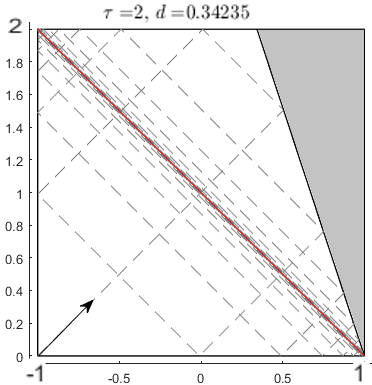
\includegraphics[scale=0.8]{Figs/CritAttrFreq.png}
    \caption{Вырожденный аттрактор внутренних волн.}
    \label{fig:trivAttr}
\end{figure}

Теперь найдем второй случай, при котором аттрактор зажимается между двумя противоположными углами. Это означает что луч пущенный из левого нижнего угла должен попасть в точку $d$. То есть $\tau = 1+d$:

\begin{equation}
    1+d=\frac{2H}{L} \sqrt{\frac{N^2}{\omega^2}-1}.
\end{equation}

Выразим отсюда частоту $\omega$:

\begin{equation}
    \omega = \frac{NH}{\sqrt{\left( 1-H\cdot tg(\alpha) \right)^2+H^2}}.
\end{equation}

После процедуры рейтрейсинга(см рис. \ref{fig:attrTriv})
    
\begin{figure}
    \centering
    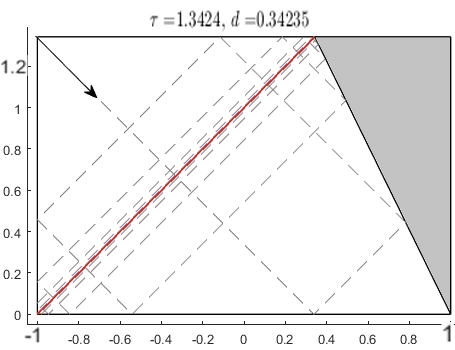
\includegraphics[scale=0.6]{Figs/AttrCritFreq.png}
    \caption{Вырожденный аттрактор внутренних волн.}
    \label{fig:attrTriv}
\end{figure}


Также с помощью метода спектральных элементов были смоделированы случаи вырожденных аттракторов (см. рис. \ref{fig:critNekfr}).

\begin{figure}
    \centering
    
    \begin{subfigure}[с]{1\textwidth}
        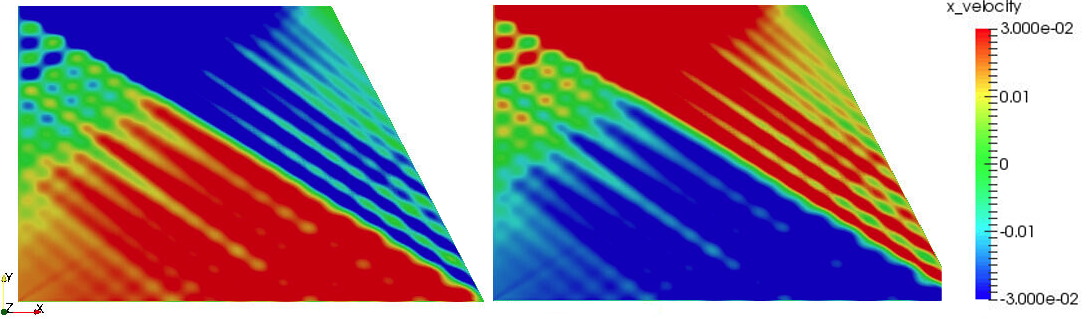
\includegraphics[scale=0.45]{Figs/AttrNEKcrit1.png}
        \caption{Расчет при помощи метода спектральных элементов с первой критической частотой}
    \end{subfigure}
    
    \begin{subfigure}[r]{1\textwidth}
        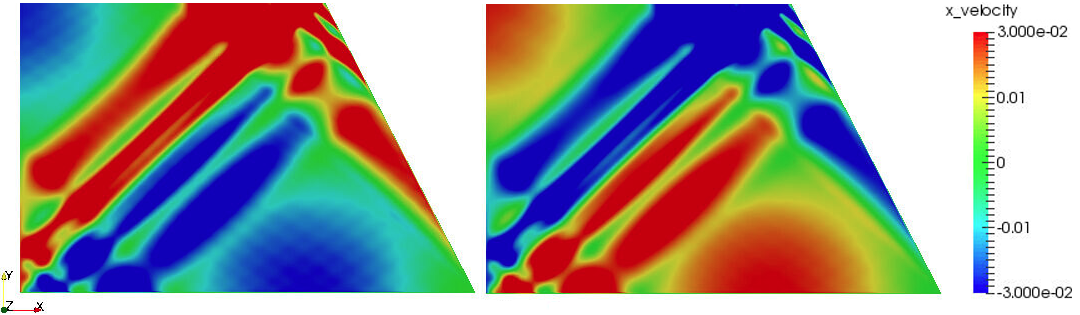
\includegraphics[scale=0.45]{Figs/AttrNekCrit2.png}
        \caption{Расчет при помощи метода спектральных элементов со второй критической частотой}
    \end{subfigure}
    \caption{Результаты расчетов при колебании волнопродуктора с критическими частотами}
    \label{fig:critNekfr}
\end{figure}

Критические значения замыкают собой диапазон частот, колебания волнопродуктора с которыми будет приводить к образованию аттрактора:

\begin{equation}
    \omega_{c_{1}}=\frac{NH}{\sqrt{L^2+H^2}}, \;\;\;\;\;\;\;\;\; \omega_{c_{2}} = \frac{NH}{\sqrt{\left( 1-H\cdot tg(\alpha) \right)^2+H^2}},
\end{equation}


\begin{equation}
    \omega_{c_{1}} \leq \omega_A \leq \omega_{c_{2}}.
\end{equation}


\section{Экспериментальные исследования}

Океан и атмосфера -- это естественные системы, обладающие стратификацией благодаря чему в них могут возникать внутренние волны. В этом разделе рассматриваются способы изучения внутренних волн в естественных условиях таких как в океане и атмосфере, а также методы воспроизвести эти условия экспериментально. Следует отметить, что в океане и атмосфере наблюдаются гравито-инерционные волны.

В лабораторных условиях рассматривается упрощенная модель, которая не учитывает эффекты связанные с вращением Земли, нелинейной стратификацией и сложной геометрией резервуара. Однако, рассматриваемые условия учитывают упрощенно основные характеристики океана. 

\subsection{Экспериментальная установка}

Экспериментальная установка представляет собой резервуар трапециевидной формы наполненный линейно стратифицированной жидкостью. Левая стенка резервуара является волнопродуктором, который производит внутренние волны. На рисунке \ref{fig:attrSetup} из \cite{Brouzet2016} изображена схема экспериментальной установки. Правая стенка наклонена на угол $\alpha$ с вертикальной стенки. Трапеция прямоугольная, с основанием $L$, высототой $H$ и глубиной $W$ вдоль оси $y$. 

\begin{figure}
    \centering
    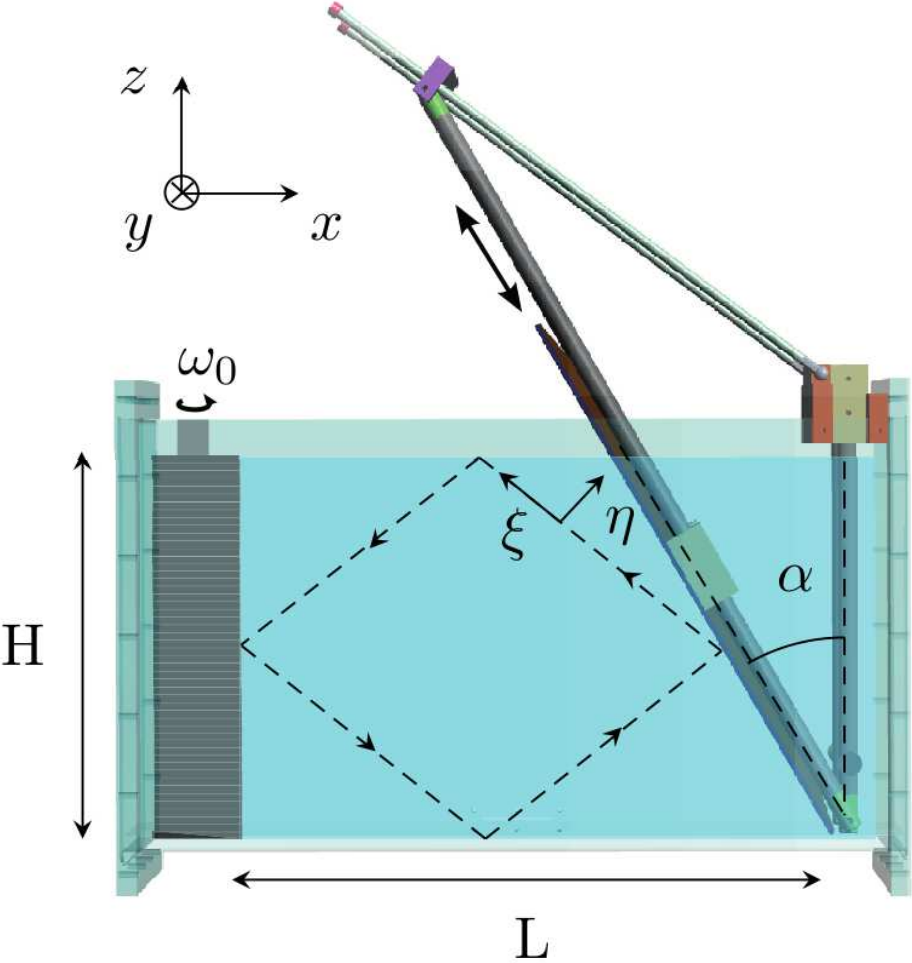
\includegraphics[scale=0.6]{pics/SetupAttr.png}
    \caption{Эксперементальная установка для воспроизведения эффекта многократной фокусировки внутренних волн. Взято из \cite{Brouzet2016}.}
    \label{fig:attrSetup}
\end{figure}

Установка для получения аттрактора внутренних волн расположена во Франции, город Лион. Внутренние волны продуцируются с помощью специального генератора. Исторически внутренние волны создавались в лаборатории путем колебания цилиндра в стратифицированной жидкости. Цилиндр создает четыре волновых луча в четырех квадрантах, как показано на рисунке \ref{fig:ermExp}. Так впервые было измерено дисперсионное соотношение для внутренних волн \cite{Grtler1943, Mowbray1967}.

Условия на левой стенке можно описать следующим уравнением:

\begin{equation}
    \zeta (z,t) = a \sin (\omega_0 t) \cos \left( \frac{\pi z}{H} \right) 
    \label{eq:wmOsc}
\end{equation}
где $a$ это амплитуда максимального смещения. 

Физически в эксперименте это достигается путем вращения дисков с эксцентриситетом в квадратных кожухах, схема изображена на рисунке. Диски размещены в разных фазах и согласованны друг с другом. Вращаясь диск сдвигает кожух, а кожух сдвигает жидкость. Профиль волнопродуктора в целом представляет собой полу косинус меняющий свою амплитуду во времени.

\begin{figure}
    \centering
    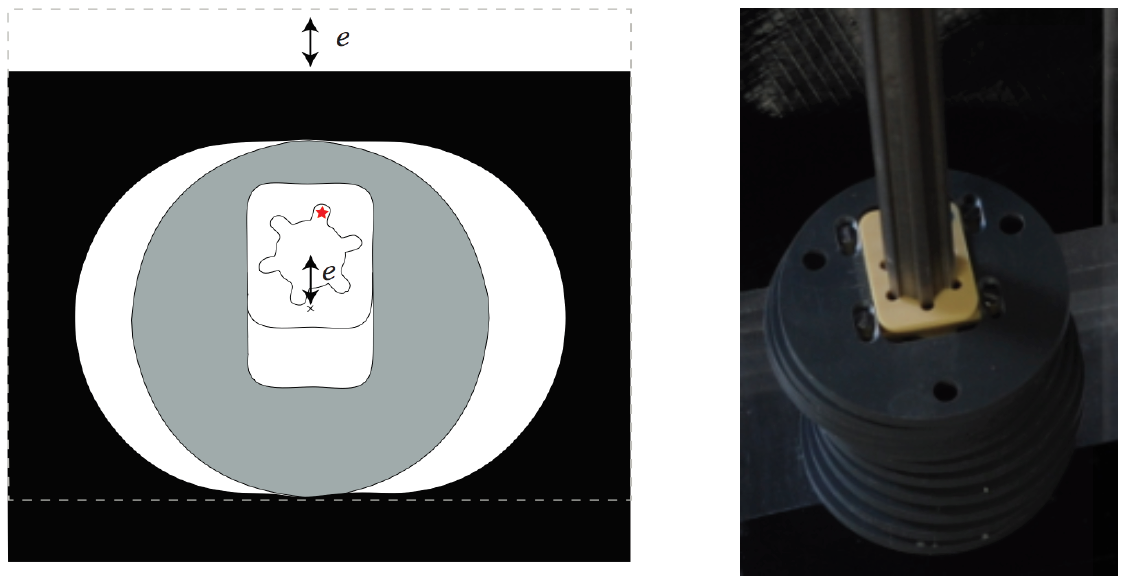
\includegraphics[scale = 0.5]{pics/wawemakerScheme.png}
    \caption{Устройство волнопродуктора для продуцирования внутренних волн в резервуаре наполненном стратифицированной жидкостью. Вращательное движение оси преобразуется в поступательное движение волнопродуктора. Изображение из \cite{Bordes2012InteractionsND, bourget, phdthesisGW}}
    \label{fig:WMrot}
\end{figure}

Такая конструкция волнопродуктора была разработана и описана в работе \cite{Gostiaux2006}, исследована \cite{MERCIER2010}, а в последствии и улучшена \cite{Bordes2012InteractionsND}. Такая конструкция позволяет очень тонко настраивать частоту амплитуду генерируемых волн.

Экспериментальная установка очень чувствительна из-за тонкой настройки стратификации. Поэтому сначала производится настройка волнопродуктора, установка фаз на дисках и амплитуд колебаний, затем резервуар заполняется водой, а потом туда аккуратно вставляется наклонная стенка под заданным углом. Регулировать после заполнения резервуара водой можно только частоту колебаний волнопродуктора. Для изменения других параметров придется заново наполнять резервуар. 

В \cite{Brouzet_2016} использовался несколько иной волнопродуктор. Идея его состоит в том, чтобы деформировать гибкую пластину, и таким образом получить закон колебания (\ref{eq:wmOsc}). На рисунке (\ref{fig:WMplate}) изображено устройство этого волнопродуктора. 

\begin{figure}
    \centering
    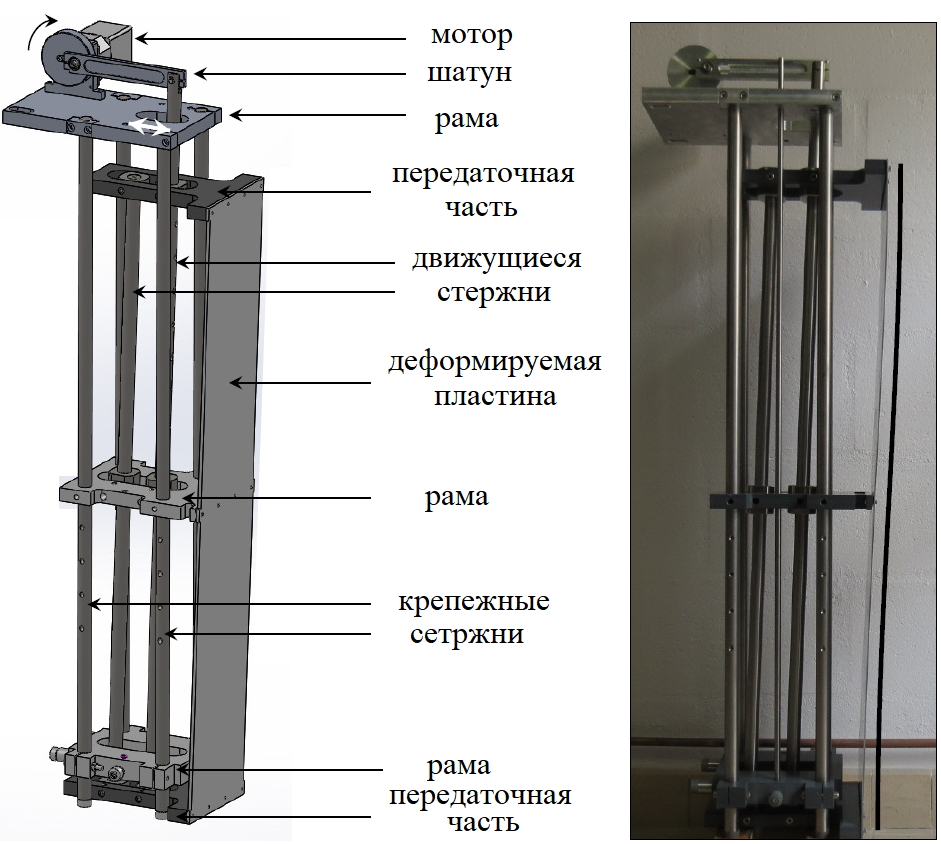
\includegraphics[scale=0.45]{pics/WMplate.png}
    \caption{Схема и фотография волнопродуктора используемого в Лионском эксперименте \cite{Brouzet_2016}}
    \label{fig:WMplate}
\end{figure}

Фиксированная часть волнопродуктора, состоит из трех различных горизонтальных частей, расположенных внизу, в середине и наверху волнопродуктора. Эти детали соединены четырьмя вертикальными стержнями. Деформируемая пластина прикреплена сверху и снизу к горизонтально перемещающимся деталям. Они движутся противофазно благодаря двум движущимся стержням по принципу деформируемого параллелограмма. Кроме того, середина пластины горизонтально прикреплена к раме, чтобы получить неподвижную точку в центре волнопродуктора. Верхняя и нижняя части двигаются поступательно благодаря двигателю в верхней части волнопродуктора. Пластина имеет ту же ширину $W$, что и резервуар, и герметизирована по бокам, чтобы избежать. Сплошная линия, имеющая форму половины косинуса, показывает, что деформация пластины очень близка к форме, которая задается формулой \ref{eq:wmOsc}. Можно изменить амплитуду колебаний, изменив стержень кривошипа после заполнения резервуара. Это позволяет проводить различные эксперименты, варьируя только амплитуду воздействия. Частоту воздействия также легко настроить, управляя двигателем.

Первые эксперименты с аттракторами внутренних волн датированы 1997 годом \cite{Maas1997}. Проведены в институте морских исследований в Нидерландах. Прямоугольный контейнер из плексигласа был заполнен экспоненциально расслоенным солевым раствором, так что частота плавучести была постоянной и составляла $N = 1.89 \; c^{-1}$. Контейнер имел трапециевидную форму в безразмерных геометрических парамерах $(\tau, d)$ $d=0$. Размеры были: глубина $(W)$ $96$ мм; высота $(H)$ $261$ мм; и длина $(L_1)$ $261$ мм. Жидкость подкрашена для визуализации внутренних волн. Краситель периодически впрыскивается в раствор, маркируя частицы жидкости заданной плотности. Вертикальная лазерная плоскость подсвечивает деформацию полосок красителя.

Внутренние волны в этом эксперименте возбуждаются колебаниями всего резервуара с частотой $\omega$ и амплитудой $a$. Тогда любая волна с частотой q параметрически усиливается. Волны повсюду возбуждаются с одинаковой фазой, задаваемой воздействием. Примерно через пять минут после начала колебания становится видимым двумерное колебательное движение линий красителя с частотой $\omega / 2$. Это колебание локализовано, принимает форму параллелограмма и наиболее ярко проявляется вокруг предсказанного с помощью трассировки лучей местоположения. 

\begin{figure}
    \centering
    \begin{subfigure}[t]{0.45\textwidth}
        \centering
        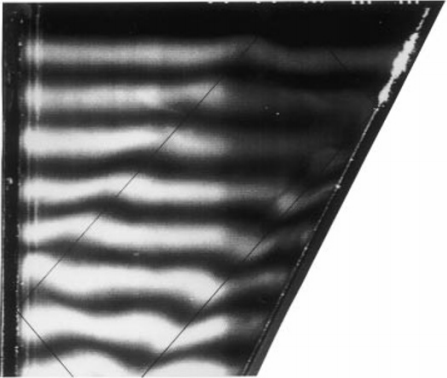
\includegraphics[scale=0.6]{pics/Exp1997Maas.png}
        \caption{предсказанная форма аттрактора с помощью метода трассировки лучей}
        \label{fig:maasExperA}
    \end{subfigure}
    \begin{subfigure}[t]{0.45\textwidth}
        \centering
        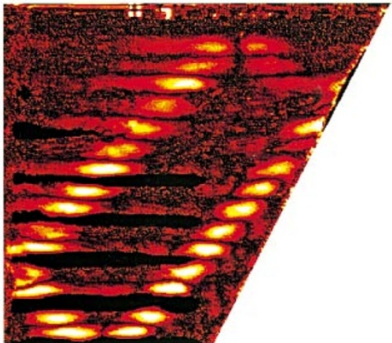
\includegraphics[scale=0.67]{pics/Exp1997MaasB.png}
        \caption{Визуализированные колебания стратифицированной жидкости после фокусировки}
        \label{fig:maasExperB}
    \end{subfigure}
    \caption{Нидерландский эксперимент проведенный Лео Маасом в 1997 году \cite{Maas1997}}
    \label{fig:maasEper1997}
\end{figure}

Затем были проведены эксперименты описанные в \cite{Brouzet_2016,Brouzet2016,brouzet1997laboratory} с волнопродукторами изображенными на рисунках \ref{fig:WMplate} и \ref{fig:WMrot}. 

В России эксперименты со стратифицированной жидкостью проводятся Евгением Ерманюком \cite{Shmakova2019}. В числе экспериментов опыты с генерированием внутренних волн \cite{Shmakova2017} и фокусировкой в тороидальном резервуаре \cite{Ermanyuk2017}.  

\section{Численные исследования}

Помимо экспериментальных исследований в лабораторных условиях проводятся и исследования численные. Одной из самых успешных практик численного моделирования аттракторов внутренних волн является моделирование при помощи метода спектральных элементов \cite{Brouzet2016} и его конкретной реализации \cite{NEK5000}. Очевидные преимущества этого метода -- скорость и точность расчетов. Недостатки также имеются.

Второй способ моделирования течения стратифицированной жидкости -- метод конечного объема и его конкретная реализация openFOAM \cite{OpenFOAM}. Попытки моделирования были проведены в 2014м году \cite{Brouzet2014}. Очевидные достоинства этого метода и реализации -- гибкость, понятность и подробная документация исходного кода. Однако и этот пусть не обделен недостатками.

В работе рассматриваются различные конфигурации расчетной области (Рис. \ref{fig:dominleft},\ref{fig:domainup}).

\begin{figure}[!ht]
        \centering
          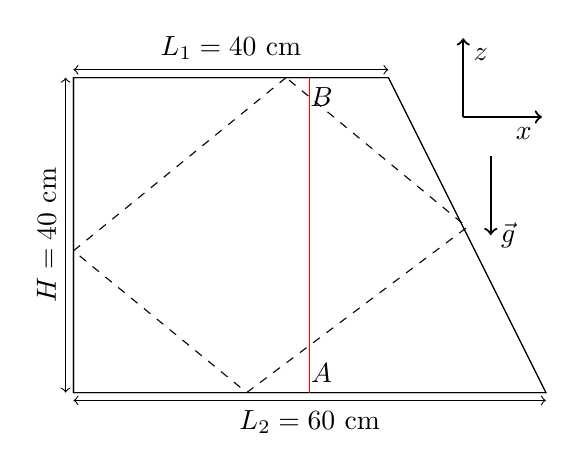
\begin{tikzpicture}[scale=1.0, z={(-.707,-.5)}]
            \draw (0,0,0) -- (6,0,0) -- (4,4,0)--(0,4,0) --cycle;
            \draw (0,0,0)     -- (6,0,0)   -- (4,4,0)   -- (0,4,0)    -- cycle;
            \draw[style = dashed] (2.7,4,0)   -- (0,1.8,0) -- (2.2,0,0) -- (5,2.1,0)-- cycle;
            %\draw[style = dashed] (0,0.985,0) -- (3.3,4,0) -- (4.5,3,0) -- (1.1,0,0)  -- cycle;

            \draw[<->] (-0.1,0) --node[above,rotate=90] {$H = 40$ cm} (-0.1,4);
            \draw[<->] (0,-0.1,0) --node[below,] {$L_2 = 60$ cm} (6,-0.1,0);
            \draw[<->] (0,4.1,0) --node[above,] {$L_1 = 40$ cm} (4,4.1,0);

            \draw[color=red] (3.0,0)--(3.0,4.0);
            
            \draw (3.15,0) node[above] {$A$};
            \draw (3.15,4.0) node[below] {$B$};

            \draw[thick,->] (4.95,3.5,0) -- (5.95,3.5,0) node[anchor=north east]{$x$};
            \draw[thick,->] (4.95,3.5,0) -- (4.95,4.5,0) node[anchor=north west]{$z$};
            \draw[thick,->] (5.3,3,0) -- (5.3,2,0) node[anchor=west]{$\vec{g}$};
          \end{tikzpicture}
          \caption{Вычислительная область для аттракторов внутренних волн, красным показана линия пробы, пунктиром показана предполагаемая форма аттрактора}
          \label{fig:dominleft}
\end{figure}

\begin{figure}[!ht]
    \centering
    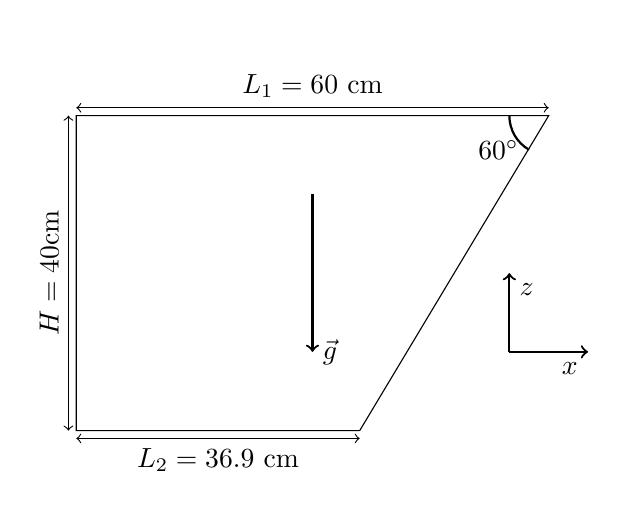
\begin{tikzpicture}[scale=1, z={(-.707,-.5)}]
    \draw (3.6,0,0) -- (0,0,0) -- (0,4,0)--(6,4,0)--(3.6,0,0);
    %\draw (3.6,0,0) -- (3.6,0,-1) -- (6,4,-1) -- (6,4,0) -- cycle;
    %\draw (6,4,0) -- (0,4,0) -- (0,4,-1) -- (6,4,-1);
    \draw (-0.5,2,0) node{};
    \draw (4.1,-.2,-1.5) node{};
    \draw (3.5,5,0) node{};
    \draw[<->] (-0.1,0) --node[above,rotate=90] {$H = 40$cm} (-0.1,4);
    \draw[<->] (0,4.1,0) --node[above,] {$L_1 = 60$ cm} (6,4.1,0);
    \draw[<->] (0,-0.1,0) --node[below,] {$L_2=36.9$ cm} (3.6,-0.1,0);
    \draw [black, thick] (5.5,4) arc [start angle=180, end angle=240, radius=0.5cm]
        node [left] {$60^\circ$};
    \draw[thick,->] (5.5,1,0) -- (6.5,1,0) node[anchor=north east]{$x$};
    \draw[thick,->] (5.5,1,0) -- (5.5,2,0) node[anchor=north west]{$z$};
    \draw[thick,->] (3,3,0) -- (3,1,0) node[anchor=west]{$\vec{g}$};
    \end{tikzpicture}
    \caption{Конфигурация вычислительной области для аттрактора внутренних гравитационных волн}
    \label{fig:domainup}
\end{figure}

Принципиальной разницы в этих двух вариантах нет в первом случае волнопродуктор располагается на левой стенке, а во втором сверху.

\subsection{Численное моделирование аттракторов внутренних волн с помощью метода спектральных элементов}

Метод спектральных элементов\cite{Patera1984}. Результаты полученные при помощи метода спектральных элементов были достаточно близки к результатам натурных экспериментов\cite{Brouzet2016,Brouzet_2016}. Недостатком метода является отсутствие реализаций с открытым исходным кодом позволяющие встроить дополнительные физические модели и проводить расчеты на сложной геометрии приближенной к реальной топологии океанического дна.

Используемая реализация -- пакет с открытым исходным кодом nek5000\cite{NEK5000}. 

В методе спектральных элементов решение и данные представлены в виде полиномов тензорного произведения $N$-го порядка внутри каждого из $E$ деформируемых шестигранных (кирпичных) элементов. Типичные дискретизации включают $E = 100 - 10 000$ элементов порядка $N = 8 - 16$ (что соответствует $512 - 4096$ точкам на элемент). Векторизация и эффективность кеширования проистекают из локального лексикографического упорядочения в каждом макроэлементе и из того факта, что действие дискретных операторов, которые номинально имеют $O(E\cdot N \cdot 6)$ ненулевых значений, может быть оценено только за $O(E\cdot N \cdot 4)$ и $O(E\cdot N\cdot 3)$. хранение за счет использования факторизации тензор-произведение-сумма. Метод спектральных элементов демонстрирует очень небольшую числовую дисперсию и диссипацию, что может быть важно, например, при расчетах устойчивости, для длительного интегрирования и для потоков с большим числом Рейнольдса.

Nek5000 решает нестационарные несжимаемые двумерные, осесимметричные или трехмерные уравнения Стокса или Навье-Стокса с вынужденной или естественной конвекцией теплопередачи как в стационарной (фиксированной), так и в движущейся геометрии. Он также решает уравнение Навье-Стокса для сжимаемой жидкости при низких числах Маха.

На данный момент это самый точный способ численно воспроизвести эксперементальные данные\cite{Brouzet2016,Brouzet_2016}. Недостаток реализации заключается в том, что геометрия задается путем аффинных преобразований. Подобрать преобразование, которое отображало бы прямоугольник в сложную геометрию океанического дна представляется трудоемкой задачей. 

Для моделирования методом спектральных элементов используется конфигурация расчетной области представленная на рисунке \ref{fig:domainup}. На протяжении всего эксперимента на верхней стенки задается граничное условие для скорости:

\begin{equation}
    U_z = A\cdot cos\left(\frac{\pi \cdot z}{L_1}\right)\cdot \omega \cdot  sin(\omega_0 t)
\end{equation}

Где $\omega_0$ -- частота волнопродуктора. 

На остальных стенках для скорости:

\begin{equation}
    \vec{U} = 0
\end{equation}

Граничные условия для давления на стенках:

\begin{equation}
    \nabla p = 0
\end{equation}

Условие для градиента солености на стенках:

\begin{equation}
    \frac{\partial s}{\partial n} = grad(s_0)
\end{equation}

$s_0$ -- начальное распределение солености в резервуаре.

\begin{figure}[!ht]
    \centering
    \begin{subfigure}[с]{0.45\textwidth}
        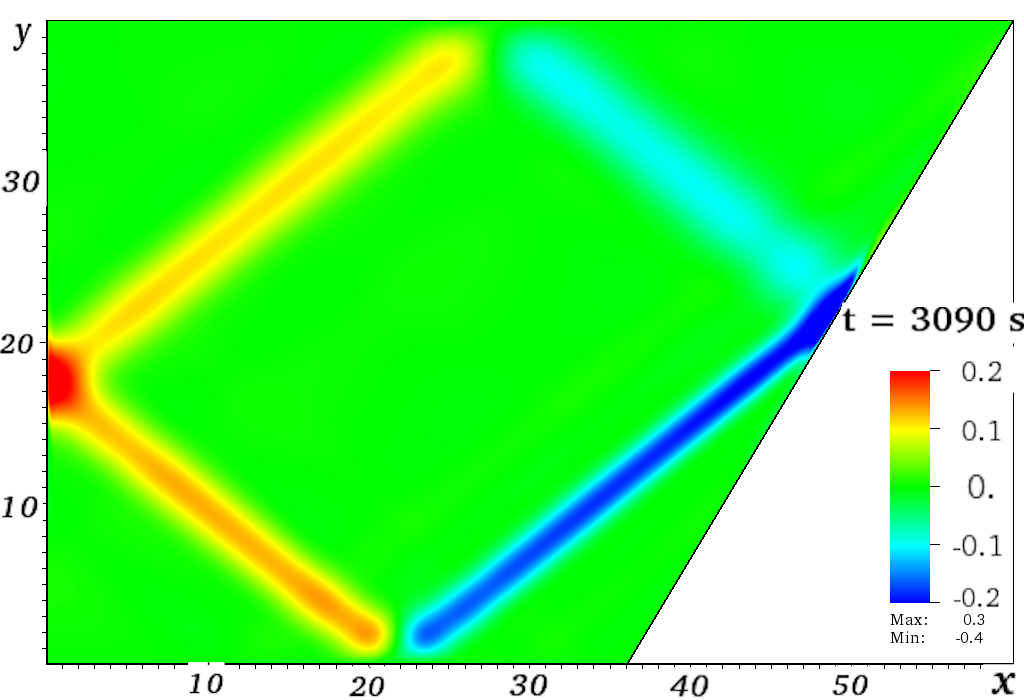
\includegraphics[scale=0.15]{pics/H40L60N1ap02dp20w0p63/2D36x36DiagramH40L60N1ap02dp20w0p63Vyn06179.png}
        \caption{Горизонтальная компонента скорости}
    \end{subfigure}
    \begin{subfigure}[с]{0.45\textwidth}
        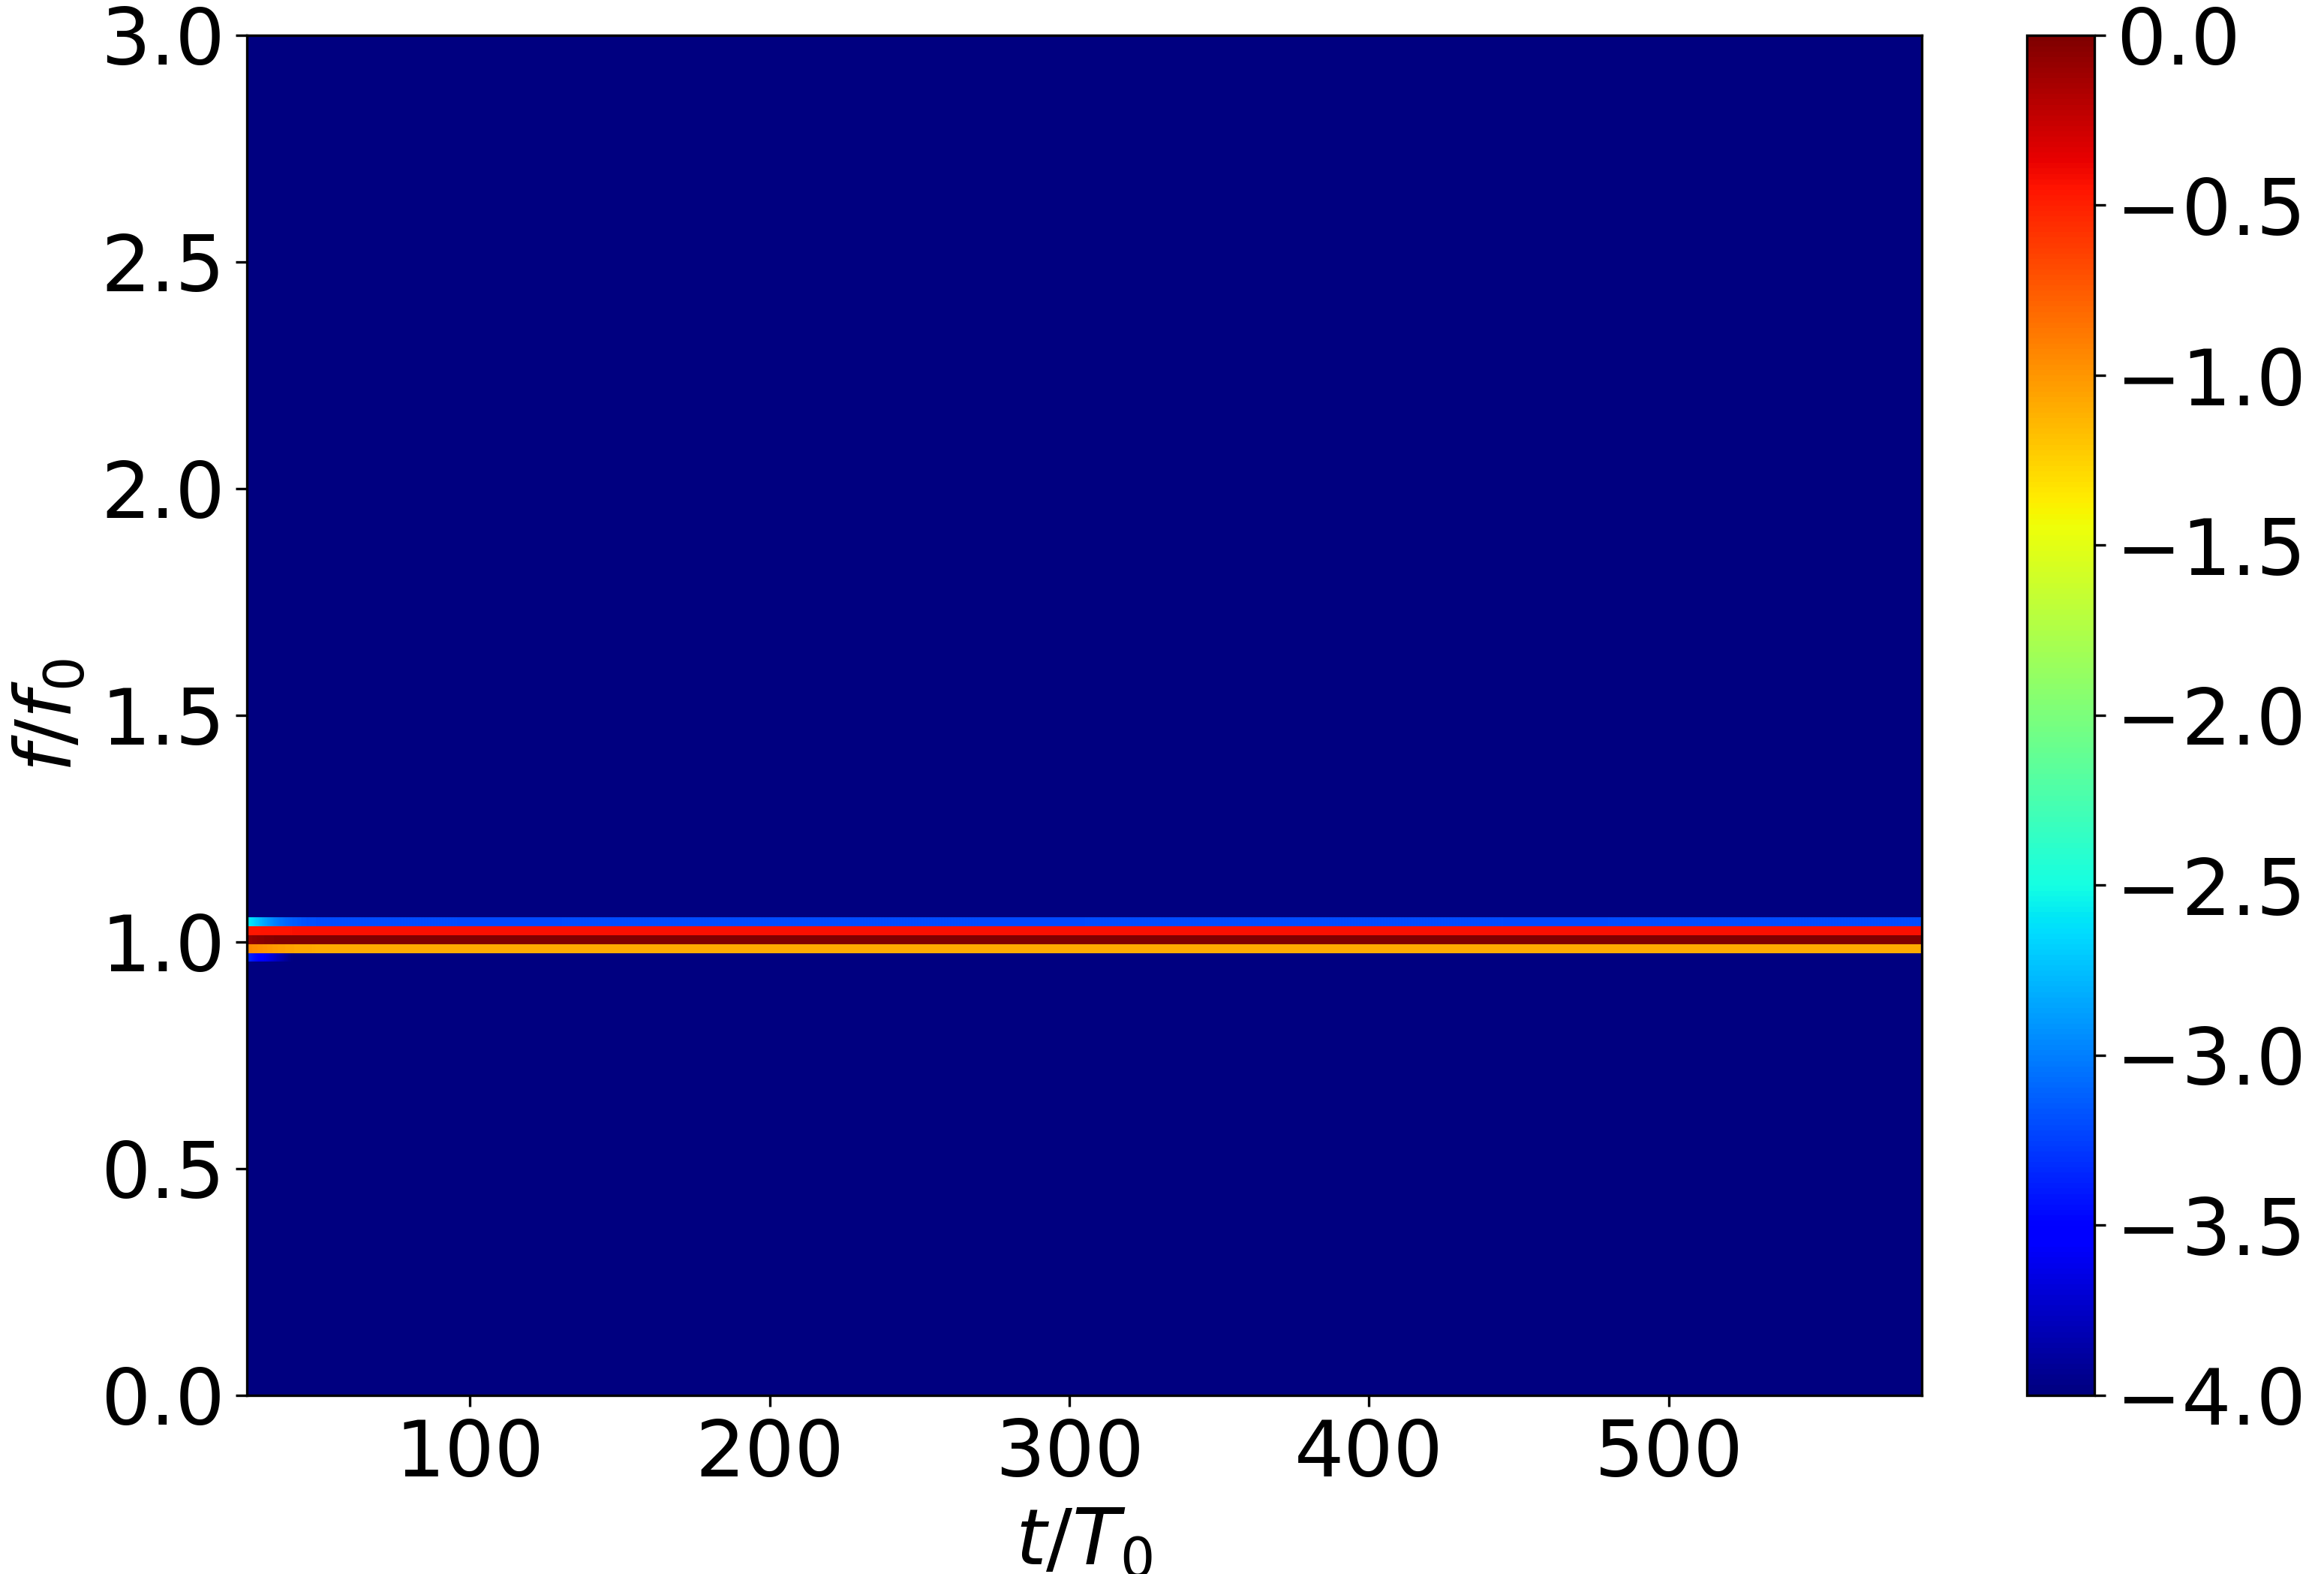
\includegraphics[scale=0.07]{pics/H40L60N1ap02dp20w0p63/TFspectrumX356Y112N1024.png}
        \caption{Частотно-временная диаграмма на аттракторе}
    \end{subfigure}
    \begin{subfigure}[с]{0.45\textwidth}
        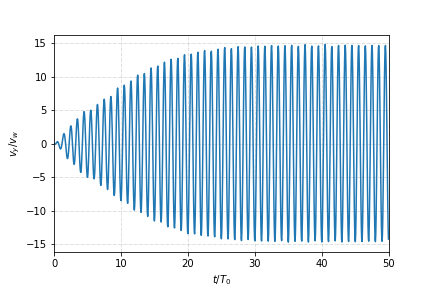
\includegraphics[scale=0.5]{pics/H40L60N1ap02dp20w0p63/vyX355662118341Y112748618745t1000.png}
        \caption{Амплитуда скорости в зависимости от времени на аттракторе}
    \end{subfigure}
    \begin{subfigure}[с]{0.45\textwidth}
        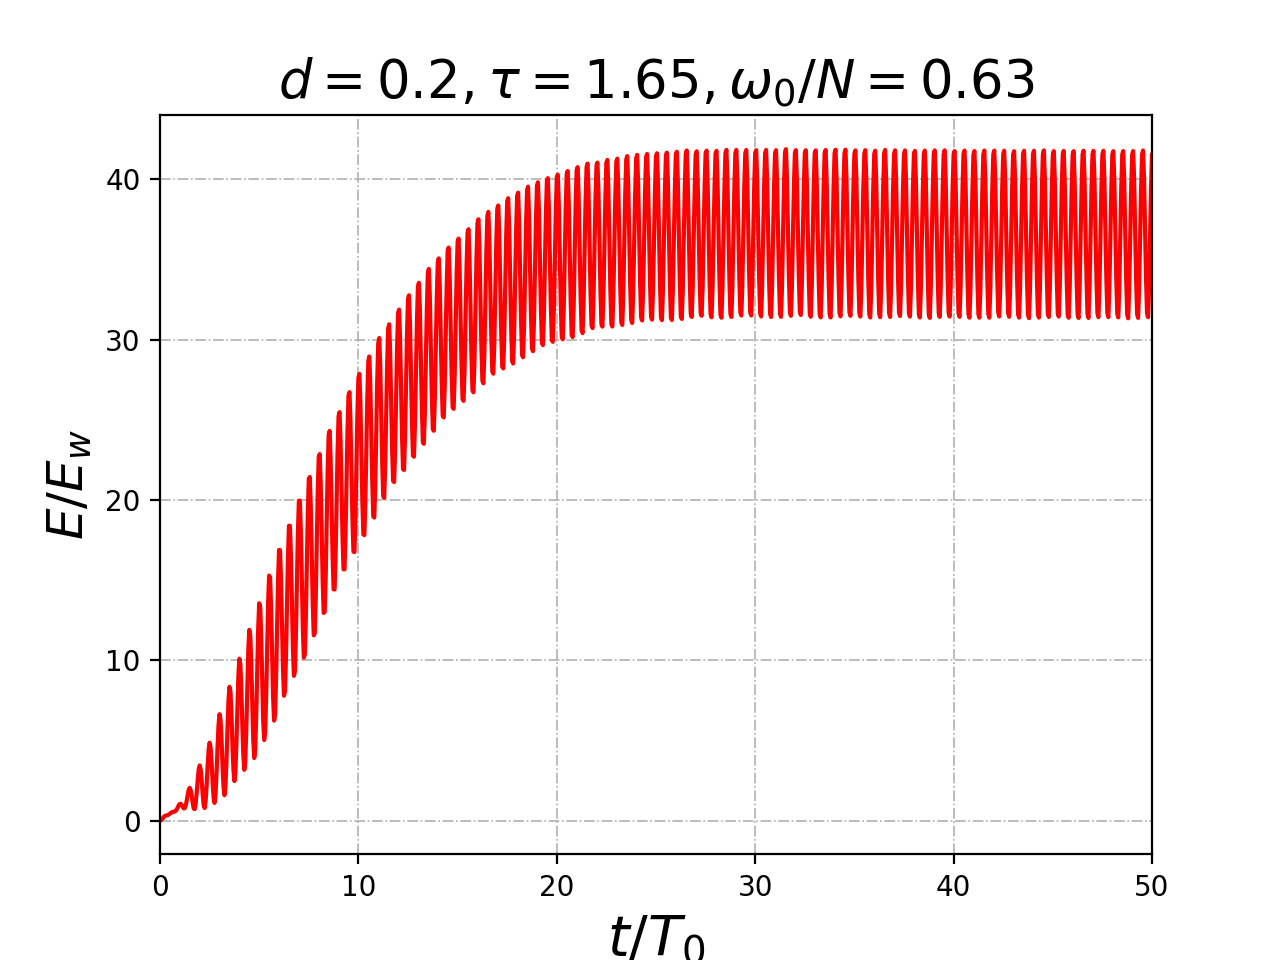
\includegraphics[scale=0.4]{pics/H40L60N1ap02dp20w0p63/2D36x36DiagramH40L60N1ap02dp20w0p63totKEnonDim.png}
        \caption{Средняя кинетическая энергия в резервуаре}
    \end{subfigure}
    
    \caption{Результат моделирования аттрактора внутренних волн методом спектральных элементов}

\end{figure}

В заключении можно сказать, что алгоритм высокого порядка точности хорошо воспроизводит результаты натурного эксперимента. В дальнейшем они будут использоваться как эталон для сравнения с остальными методами решения. 

\subsection{Численное моделирование аттракторов внутренних волн с помощью метода контрольного объема}

Для моделирования методом конечного объема используется конфигурация представленная на рисунке \ref{fig:dominleft} в этом случае волнопродуктор установлен на левой стенке и колеблется по следующему правилу:

\begin{equation}
    U_x = A\cdot cos\left(\frac{\pi \cdot z}{H}\right)\cdot \omega \cdot  sin(\omega_0 t)
\end{equation}

Аналогично условия на остальных стенках:

\begin{equation}
    \vec{U} = 0
\end{equation}

Для далвения:

\begin{equation}
    \nabla p = 0
\end{equation}

Для градиента солености:

\begin{equation}
    \frac{\partial s}{\partial n} = grad(s_0)
\end{equation}

Уравнения движения стратифицированной жидкости (\ref{eq:momClassic} - \ref{eq:contClassic}) представляются в виде дискретных аналогов. Аналог производной по времени:

\begin{equation}\label{eq:qhd_Euler}
    \frac{\partial \vec{U}}{\partial t} \approx \frac{ \vec{U}^n-\vec{U}^o}{\Delta t}, \,\,\,  \frac{\delta \vec{U}}{\delta t} =  \frac{ \vec{U}^n-\vec{U}^o}{\Delta t},
\end{equation}
разностный аналог уравнения движения:

\begin{multline}\label{eq:qhd_approx_momentum}
    \frac{\delta \vec{U}}{\delta t} + \frac{1}{V} \sum_f \vec{S}_f \cdot \vec{U}^o_f \otimes \vec{U}^n_f  - \frac{1}{V} \sum_f \nu_f \frac{\delta\vec{U}^n}{\delta \vec{n}_f} |\vec{S}_f| - \frac{1}{V} \sum_f \nu_f \vec{S}_f \cdot [\nabla \vec U^o]_f^T = \\
    = - \frac{1}{\rho_0} \frac{1}{V} \sum_f \tilde p^o_f \vec S_f + \vec{F}^o,
\end{multline}
и аналог уравнения неразрывности:

\begin{equation}
    \sum_f \vec{S_f} \cdot \vec{U}_f^n = 0.
\end{equation}

Производные по направлению вычисляются согласно шаблону приведённому на рис. \ref{qhd}:

\begin{equation}
    \vec{U}_w^n= \frac{\vec{U}_W^n-\vec{U}_P^n}{|\vec{d}_f|}|\vec{d}|+\vec{U}_P, \,\,\, \frac{\delta\vec{U}^n}{\delta \vec{n}_w} = \frac{\vec{U}^n_P-\vec{U}^n_W}{|\vec{d}|},
\end{equation}

\begin{figure}
    \centering
    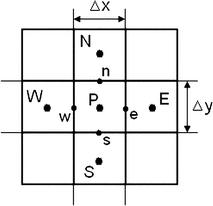
\includegraphics{pics/b701170a-f6.jpeg}
    \caption{Расчетный шаблон для метода конечных элементов}
    \label{qhd}
\end{figure}

В качестве алгоритма нахождения численного решения используется PISO \cite{IssaGosmanWatkins-PISO}. Вкратце изложить алгоритм нахождения полей скорости и давления можно так:

\begin{enumerate}[1.]
    \item Устанавливаются граничные условия.
    \item Решается дискредитированное уравнение движения для вычисления промежуточных значений поля скорости.
    \item Вычисляются массовые потоки через границы ячеек.
    \item Решается уравнение для давления.
    \item Корректируются массовые потоки.
    \item Корректируется поле скорости согласно новому давлению.
    \item Обновляются граничные условия.
    \item Вернуться к третьему шагу.
    \item Перейти на следующий временной шаг и начать с первого пункта.
\end{enumerate}

Внутри шага по времени имеется цикл между пунктом 3 и пунктом 8. Более того возможны коррекции неортогональности ячеек сетки если зациклить этот алгоритм между пунктом 4 и 5. дискредитированное уравнение движение в матричном виде можно записать следующим образом: 

\begin{equation}
    \left[
        \begin{array}{cccc}
            m_{11} & m_{12} & \ldots & m_{1n}\\[0.055cm]
            m_{21} & m_{22} & \ldots & m_{2n}\\[0.055cm]
            \vdots & \vdots & \ddots & \vdots\\[0.055cm]
            m_{n1} & m_{n2} & \ldots & m_{nn}
        \end{array}
        \right]
        \left[
        \begin{array}{c}
            \vec{U}_{1}^* \\[0.1cm] 
            \vec{U}_{2}^* \\[0.1cm]
            \vdots \\[0.1cm]
            \vec{U}_{n}^*  
        \end{array}
        \right]
        =
        \left[
        \begin{array}{c}
            \vec{R}_{1} \\[0.1cm] 
            \vec{R}_{2} \\[0.1cm]
            \vdots \\[0.1cm]
            \vec{R}_{n}  
        \end{array}
    \right],
\end{equation}

или в полудискретной записи:

\begin{equation}
    \mathcal{M} \vec{U}^* = -\frac{\nabla p}{\rho_m} + \vec{F}.
\end{equation}

Где матрица  $\mathcal{M}$ состоит из коэффициентов   которые вычисляются как сумма потоков через соответствующие грани контрольного объема. $\vec{U}^*$ -- искомые промежуточные значения поля скоростей. Для получения уравнения давления эта матрица коэффициентов расщепляется следующим образом:

\begin{equation}
    \left[
        \begin{array}{cccc}
            m_{11} & m_{12} & \ldots & m_{1n}\\[0.055cm]
            m_{21} & m_{22} & \ldots & m_{2n}\\[0.055cm]
            \vdots & \vdots & \ddots & \vdots\\[0.055cm]
            m_{n1} & m_{n2} & \ldots & m_{nn}
        \end{array}
        \right]
        \left[
        \begin{array}{c}
            \vec{U}_{1}^* \\[0.1cm] 
            \vec{U}_{2}^* \\[0.1cm]
            \vdots \\[0.1cm]
            \vec{U}_{n}^*  
        \end{array}
        \right]
        =
        \left[
        \begin{array}{c}
            \vec{H}_{1} \\[0.1cm] 
            \vec{H}_{2} \\[0.1cm]
            \vdots \\[0.1cm]
            \vec{H}_{n}  
        \end{array}
        \right]
        -
        \left[
        \begin{array}{c}
            \frac{\nabla p_1}{\rho_m} \\[0.1cm] 
            \frac{\nabla p_2}{\rho_m} \\[0.1cm]
            \vdots \\[0.1cm]
            \frac{\nabla p_n}{\rho_m}
        \end{array}
        \right],
\end{equation}

или в полудискретной записи:

\begin{equation}
    \mathcal{M} \vec{U}^* = \mathcal{A} \vec{U}^* - \mathcal{\vec{H}},
\end{equation}
где $\mathcal{\vec{H}}$ -- источниковые члены для уравнения давления. $\mathcal{A}=diag(\mathcal{M})$. Подставляем расщепленную матрицу коэффициентов в уравнение движение:
\begin{equation}
    \mathcal{A} \vec{U}^* - \mathcal{\vec{H}}= -\frac{\nabla p}{\rho_m} + \vec{F}    
\end{equation}
Умножаем обе части на $\mathcal{A}^{-1}$, выражаем $\vec U$

\begin{equation}
    \mathcal{A}^{-1} \mathcal{A} \vec{U} = \mathcal{A}^{-1} \mathcal{\vec{H}} - \mathcal{A}^{-1} \nabla p + \mathcal{A}^{-1} \vec{F} \;\;=>\;\;
    \vec{U} = \mathcal{A}^{-1} \mathcal{\vec{H}} - \mathcal{A}^{-1} \nabla p + \mathcal{A}^{-1} \vec{F}
\end{equation}
согласно уравнению неразрывности $\nabla \vec{U} = 0$, это дает нам уравнение для давления:

\begin{equation}
    \nabla \cdot (\mathcal{A}^{-1} \nabla p) = \nabla \cdot (\mathcal{A}^{-1} \mathcal{\vec{H}} + \mathcal{A}^{-1} \vec{F})
\end{equation}

Алгоритм PISO не прост в понимании и сложен из-за двух вложенных циклов внутри одного временного шага. Но очень популярен и долгое время остается одним из самых востребованных инструментов вычислительной  гидродинамики. Блок-схема алгоритма проиллюстрирована на рис. \ref{fig:blockSchemePIMPLE}

\begin{figure}[h]
    \tikzstyle{decision} = [diamond, draw, 
    text width=4.5em, text badly centered, node distance=2cm, inner sep=0pt, minimum width=10em]
    \tikzstyle{block} = [rectangle, draw
    %, text width=30em
    , text centered, minimum height=2em, node distance=1.5cm
    %,minimum width=30em
    ]
    \tikzstyle{line} = [draw, -latex']
    \tikzstyle{cloud} = [draw, ellipse,fill=red!20, node distance=4cm,
    minimum height=2em]
    \centering
    \begin{tikzpicture}[node distance = 2cm, auto,scale = 1]
    % Place nodes
        \node [block] (UpdateF) {Начало};
        
        \node [block, below of=UpdateF] (Control) {Вчисление потоков};
        \node [block, below of=Control] (Stability) {Решение уравнения движения};
        \node [block, below of=Stability] (Increasing) {Решение уравнения давления с учетом неортогональности};
        \node [block, below of=Increasing] (Store) {Обновление давления и скорости};

        \node [decision, below of=Store] (Pressure) {PISO?};
        \tikzstyle{block} = [rectangle, draw, text centered, minimum height=2em, node distance=2.5cm]
        \node [block, below of=Pressure] (Salinity) {Обновление оператора при уравнении движения};
        
        \tikzstyle{block} = [rectangle, draw, text centered, minimum height=2em, node distance=1.5cm]    
        
        \node [block, below of=Salinity] (SolvePressure) {Решение уравнения давления с учетом неортогональности};
        

        %\tikzstyle{decision} = [diamond, aspect=2,draw, text width=10em, text badly centered, node distance=2cm, inner sep=0pt, minimum width=2em,minimum height=2em]
       % \node [decision, below of=Salinity] (NoNOrth) {Non-orthogonal corrections?};
        \tikzstyle{block} = [rectangle, draw, text centered, minimum height=2em, node distance=1.7cm]
        \node [block, below of=SolvePressure] (pressureUpd) {Обновление давления и скорости};
        \tikzstyle{block} = [rectangle, draw, text centered, minimum height=2em, node distance=1.7cm]
        \node [block, below of=pressureUpd] (solveOther) {Решение уравнения переноса};
        
        \node [decision, below of=solveOther] (conv){Сошлось?};
        \tikzstyle{block} = [rectangle, draw, text centered, minimum height=2em, node distance=2.5cm]
        \node [block, below of=conv] (end) {Конец};
        \tikzstyle{block} = [rectangle, draw, text centered, minimum height=2em, node distance=2cm]


        \path [line,distance = 5cm] (UpdateF) -- (Control);
        \path [line] (Control) -- (Stability);
        \path [line] (Stability) -- (Increasing);
        \path [line] (Increasing) -- (Store);
        \path [line] (Store) -- (Pressure);
        \path [line] (Pressure) -- node {да} (Salinity);
        \path [line] (Pressure) -| node [near start] {нет} ($(solveOther.west)-(4,0)$) -- (solveOther.west);

        %\path [line] (Salinity) -- (pressureUpd);
        \path [line] (Salinity) -- (SolvePressure);
        \path [line] (SolvePressure) -- (pressureUpd);
        %\path [line] (NoNOrth) -- node {no} (pressureUpd);
        %\path [line] (NoNOrth) -| node[near start] {yes} ($(Increasing.east)+(2,0)$) -- (Increasing.east);
        \path [line] (pressureUpd) -- (solveOther);
        \path [line] (solveOther) -- (conv);
        \path [line] (conv) -- node {да} (end);
        \path [line] (conv) -| node[near start] {нет} ($(Control.east)+(5,0)$) -- (Control.east);
        %path [line] (setValues.north) -| ($(Control.east)+(1.45,0)$) -- (Control.east);
    \end{tikzpicture}
    
    \caption{Схема алгоритма PISO}
    \label{fig:blockSchemePIMPLE}
\end{figure}

К сожалению, результаты моделирования аттрактора внутренних волн алгоритмом PISO количественно не соответствуют результатам полученным при помощи метода спектральных элементов. 

Подведя итог можно сказать следующее, популярный алгоритм качественно воспроизводит картину течения, образующуюся при многократном отражении внутренних волн от стенок трапециевидного резервуара. Но количественно нет. Преимуществом алгоритма является способность работать с неортогональными сетками и сложной геометрией. К недостаткам можно отнести сложность и нелинейность процедуры нахождения гидродинамических полей.

\begin{figure}[!ht]
    \centering
        \begin{tikzpicture}[scale=5.34, z={(-.707,-.5)}]
          \node[anchor=south west,inner sep=0] at (0,0) {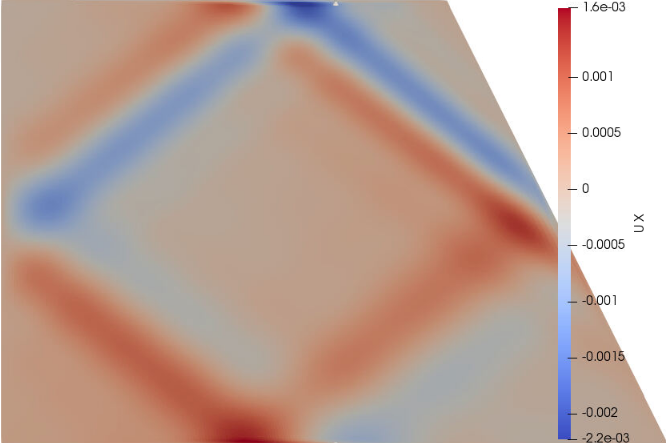
\includegraphics[width=\textwidth]{Figs/Attr200s.png}};
          \draw[thick,style = dashed] (1.5, 0, 0) -- (1.5, 2, 0);
        \end{tikzpicture}
    \caption{Поле горизонтальной компоненты скорости, пунктиром показана линия пробы}
    \label{fig:attractorRes}
\end{figure}

\begin{figure}[!ht]
    \centering
            \begin{tikzpicture}[scale = 1]
            \begin{axis}
                [scale only axis, grid=major,legend style={at={(0,1),font=\LARGE},anchor=north west}, ymin=-0.8*10^-3, ymax=1.7*10^-3,legend style={nodes={scale=0.5, transform shape}}, x post scale=1.6,xlabel={$y$}, ylabel={$U_x$}]

                \addplot[solid,color=red,thick] table [x=Points:1, y=Result, col sep=comma] {CSV/snappy180x180nCor4NonOrth4.csv};

                \addplot[solid,color=blue,thick] table [x=Points:1, y=Result, col sep=comma] {CSV/FVMnocor.csv};

                \addplot[solid,color=orange,thick,dashed] table [x=Points:1, y=Result, col sep=comma] {CSV/FVM450x2.csv};

                \legend{PISO 225x150*, PISO 225x150, PISO 450x300}
            \end{axis}
            \begin{axis}
                [scale only axis, ymin=-0.8*10^-1, ymax=1.7*10^-1, yticklabels={,,},xticklabels={,,},legend style={at={(0,0.76),font=\LARGE},anchor=north west},legend style={nodes={scale=0.5, transform shape}},x post scale=1.6]
%                \addplot[solid,thick] table [x=Points:1, y=x_velocity, col sep=comma] {CSV/Ux30Nek500T200.csv};
                \legend{NEK5000}
            \end{axis}
        \end{tikzpicture} 
    \caption{Результат моделирования с помощью алгоритма PISO, отсутствие сеточной сходимости. звёздочкой отмечены результаты моделирования с дополнительными коррекциями.}
    \label{fig:PISOattr}
\end{figure}

\begin{figure}
    \centering
        \begin{tikzpicture}[scale = 1.1]
          \begin{axis}
             [scale only axis, grid=major,legend style={at={(0.3,1),font=\LARGE},anchor=north west}, ymin=-1.2*10^-3, ymax=1.7*10^-3, xmin=0.0,legend style={nodes={scale=0.5, transform shape}}, x post scale=1.5,xlabel={$y$}, ylabel={$U_x$}];

            \addplot[solid,thick, color=orange, dashed] table [x=y, y=U_0m, col sep=comma]
            {CSV/U225x300A01w623corr31300_U.csv};
            \addplot[solid,thick, color=cyan] table [x=y, y=U_0m, col sep=comma]
            {CSV/U300x450A01w623corr31300_U.csv};
            \addplot[solid,thick, color=blue] table [x=y, y=U_0m, col sep=comma]
            {CSV/U450x600A01w623corr31300_U.csv};

            \legend{PISO 225x300,PISO 300x450,PISO 450x600}
          \end{axis}
          \begin{axis}
            [scale only axis, ymin=-1.2*10^-1, ymax=1.7*10^-1, xmin=0.0,  yticklabels={,,},xticklabels={,,},legend style={at={(0.3,0.8),font=\LARGE},anchor=north west},legend style={nodes={scale=0.5, transform shape}},x post scale=1.5];
            \addplot[solid,thick, color = red] table [x=Points:1, y=x_velocity, col sep=comma] {CSV/NEK300s0.csv};
            \legend{NEK 5000}
          \end{axis}
        \end{tikzpicture}
    \caption{Сравнение горизонтальной компоненты скорости полученной при различных размерах расчетной сетки для алгоритма PISO с той же величиной полученной при помощи метода спектральных элементов.  Время = 300 с.}
    \label{fig:meshAttr300PISO}
\end{figure}

